% Generated by LitigCharts.WorkedPathDiagram. Edit its C# layout, not this output.
% All empirical probabilities, utilities, information-set numbers and payoffs
% are loaded from the extraction. See the accompanying .txt for interpretation.
\documentclass[10pt,tikz,border=4pt]{standalone}
\usepackage{amsmath}
\usepackage{lmodern}
\usetikzlibrary{arrows.meta,calc,positioning}
% Generated numerical bindings. Do not edit these values by hand.
\newcommand{\AnswerInfo}{12}
\newcommand{\AnswerUtility}{9.503}
\newcommand{\CourtLoseProbability}{0.813}
\newcommand{\CourtWinProbability}{0.187}
\newcommand{\DExitInfo}{13}
\newcommand{\DSignalAdjacentProbability}{0.156}
\newcommand{\DSignalMainProbability}{0.157}
\newcommand{\DSignalMixedProbability}{0.182}
\newcommand{\DemandLowDeviationUtility}{9.900}
\newcommand{\DemandLowValue}{0.05}
\newcommand{\DemandMainInfo}{55}
\newcommand{\DemandMainUtility}{9.936}
\newcommand{\DemandMainValue}{0.75}
\newcommand{\DemandMixedInfo}{51}
\newcommand{\DemandMixedUtility}{9.900}
\newcommand{\FileMainInfo}{52}
\newcommand{\FileMainUtility}{10.099}
\newcommand{\FileMixedInfo}{48}
\newcommand{\FileMixedProbability}{0.878}
\newcommand{\FileMixedUtility}{10.000}
\newcommand{\HighDeviationPayoff}{0.60,\,-0.90}
\newcommand{\LowDeviationPayoff}{-0.10,\,-0.20}
\newcommand{\NoAnswerPayoff}{0.85,\,-1.00}
\newcommand{\NoAnswerUtility}{9.000}
\newcommand{\NoFileMainUtility}{10.000}
\newcommand{\NoFileMixedProbability}{0.122}
\newcommand{\NoFileMixedUtility}{10.000}
\newcommand{\NoFilingPayoff}{0.00,\,0.00}
\newcommand{\OfferHighUtility}{9.245}
\newcommand{\OfferInfo}{15}
\newcommand{\OfferUtility}{9.503}
\newcommand{\OfferValue}{0.05}
\newcommand{\PExitMainInfo}{53}
\newcommand{\PExitMixedInfo}{49}
\newcommand{\SettlementPayoff}{-0.10,\,-0.20}
\newcommand{\SignalMainProbability}{0.108}
\newcommand{\SignalMixedProbability}{0.106}
\newcommand{\TrialDCost}{0.30}
\newcommand{\TrialLosePayoff}{-0.30,\,-0.30}
\newcommand{\TrialPCost}{0.30}
\newcommand{\TrialTransfer}{1.00}
\newcommand{\TrialWinPayoff}{0.70,\,-1.30}

\begin{document}
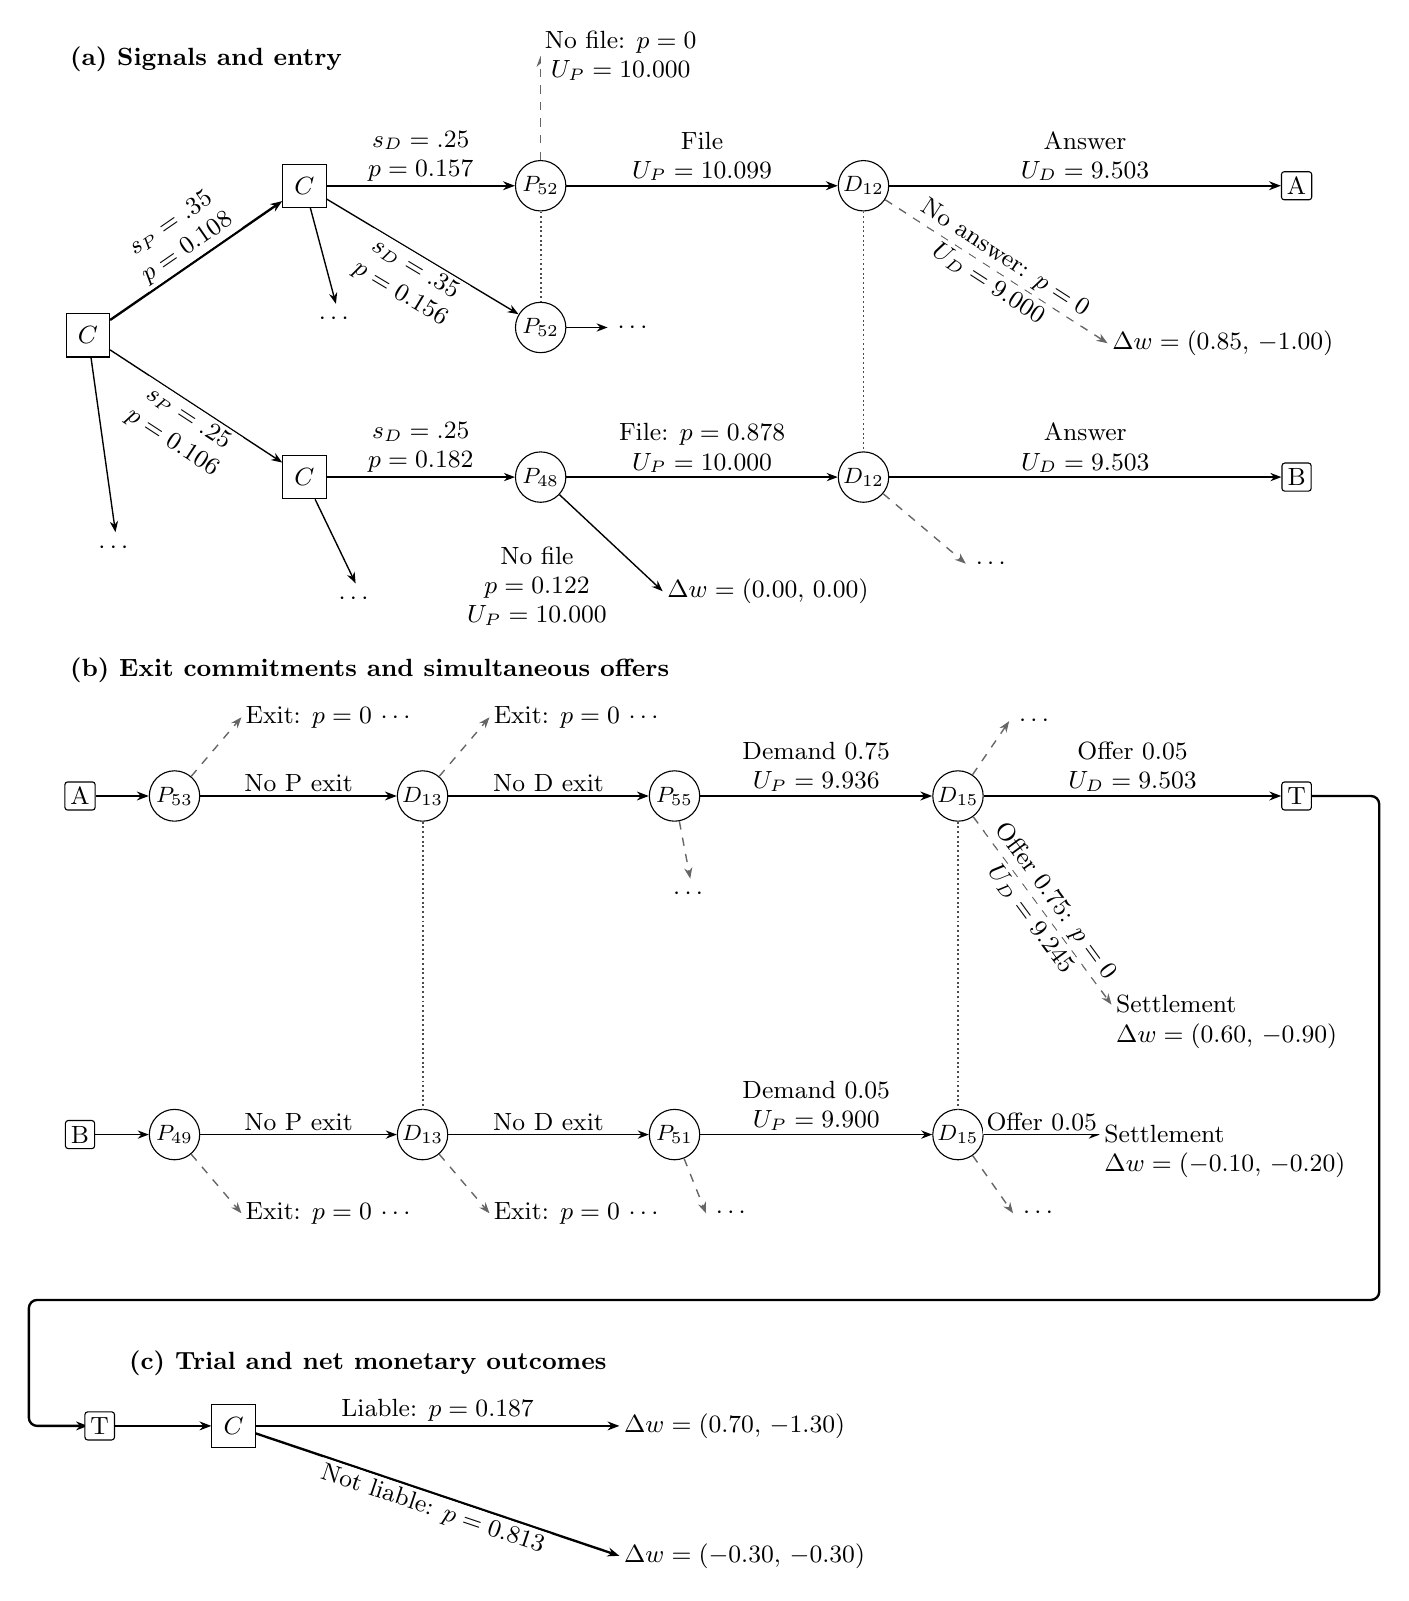
\begin{tikzpicture}[x=1cm,y=1cm,font=\fontsize{9}{10.5}\selectfont,
  player/.style={circle,draw,fill=white,minimum size=6.4mm,inner sep=0pt,font=\fontsize{8.5}{9}\selectfont},
  chance/.style={rectangle,draw,fill=white,minimum size=5.5mm,inner sep=0pt},
  main/.style={-{Stealth[length=1.5mm]},line width=0.85pt},
  branch/.style={-{Stealth[length=1.4mm]},line width=0.5pt},
  deviation/.style={branch,dashed,draw=black!60},
  infoset/.style={densely dotted,draw=black!70,line width=0.7pt},
  lab/.style={fill=white,inner sep=1.3pt,align=center},
  payoff/.style={align=left,anchor=west,inner sep=1.5pt},
  cont/.style={draw,rounded corners=1pt,fill=white,inner sep=2pt,font=\small},
  stage/.style={anchor=west,font=\small\bfseries}]

% (a) Two adjacent plaintiff signals; one additional defendant signal makes
% the plaintiff's imperfect information visible without expanding that subtree.
\node[stage] at (-0.1,0.6) {(a) Signals and entry};
\node[chance] (root) at (0.25,-2.9) {$C$};
\node[chance] (cdh) at (3,-1) {$C$};
\node[chance] (cdl) at (3,-4.7) {$C$};
\node[player] (pfh) at (6,-1) {$P_{\FileMainInfo}$};
\node[player] (pfalt) at (6,-2.8) {$P_{\FileMainInfo}$};
\node[player] (pfl) at (6,-4.7) {$P_{\FileMixedInfo}$};
\node[player] (dah) at (10.1,-1) {$D_{\AnswerInfo}$};
\node[player] (dal) at (10.1,-4.7) {$D_{\AnswerInfo}$};
\node[cont] (aend) at (15.6,-1) {A};
\node[cont] (bend) at (15.6,-4.7) {B};

\draw[main] (root) -- node[lab,above,sloped] {$s_P=.35$\\$p=\SignalMainProbability$} (cdh);
\draw[branch] (root) -- node[lab,below,sloped] {$s_P=.25$\\$p=\SignalMixedProbability$} (cdl);
\draw[branch] (root) -- (0.6,-5.4) node[below] {$\cdots$};
\draw[main] (cdh) -- node[lab,above] {$s_D=.25$\\$p=\DSignalMainProbability$} (pfh);
\draw[branch] (cdh) -- node[lab,below,sloped] {$s_D=.35$\\$p=\DSignalAdjacentProbability$} (pfalt);
\draw[branch] (cdh) -- (3.4,-2.5) node[below] {$\cdots$};
\draw[infoset] (pfh) -- (pfalt);
\draw[branch] (pfalt) -- (6.85,-2.8) node[right] {$\cdots$};
\draw[branch] (cdl) -- node[lab,above] {$s_D=.25$\\$p=\DSignalMixedProbability$} (pfl);
\draw[branch] (cdl) -- (3.65,-6.05) node[below] {$\cdots$};

\draw[main] (pfh) -- node[lab,above] {File\\$U_P=\FileMainUtility$} (dah);
\draw[deviation] (pfh) -- (6,0.65) node[lab,right] {No file: $p=0$\\$U_P=\NoFileMainUtility$};
\draw[branch] (pfl) -- node[lab,above] {File: $p=\FileMixedProbability$\\$U_P=\FileMixedUtility$} (dal);
\draw[branch] (pfl) -- (7.55,-6.15)
  node[lab,pos=0.5,below left] {No file\\$p=\NoFileMixedProbability$\\$U_P=\NoFileMixedUtility$};
\node[payoff] at (7.55,-6.15) {$\Delta w=(\NoFilingPayoff)$};
\draw[infoset] (dah) -- (dal);
\draw[branch] (dal) -- node[lab,above] {Answer\\$U_D=\AnswerUtility$} (bend);
\draw[deviation] (dah) --
  node[lab,pos=0.5,above,sloped] {No answer: $p=0$}
  node[lab,pos=0.5,below,sloped] {$U_D=\NoAnswerUtility$} (13.2,-3);
\node[payoff] at (13.2,-3) {$\Delta w=(\NoAnswerPayoff)$};
\draw[main] (dah) -- node[lab,above] {Answer\\$U_D=\AnswerUtility$} (aend);
\draw[deviation] (dal) -- (11.4,-5.8) node[right] {$\cdots$};

% (b) Repeated D nodes and dotted connections are essential: neither the
% opponent's private signal nor the simultaneous action becomes observed.
\node[stage] at (-0.1,-7.15) {(b) Exit commitments and simultaneous offers};
\node[cont] (astart) at (0.15,-8.75) {A};
\node[player] (pexh) at (1.35,-8.75) {$P_{\PExitMainInfo}$};
\node[player] (dexh) at (4.5,-8.75) {$D_{\DExitInfo}$};
\node[player] (poh) at (7.7,-8.75) {$P_{\DemandMainInfo}$};
\node[player] (doh) at (11.3,-8.75) {$D_{\OfferInfo}$};
\node[cont] (tend) at (15.6,-8.75) {T};
\node[cont] (bstart) at (0.15,-13.05) {B};
\node[player] (pexl) at (1.35,-13.05) {$P_{\PExitMixedInfo}$};
\node[player] (dexl) at (4.5,-13.05) {$D_{\DExitInfo}$};
\node[player] (pol) at (7.7,-13.05) {$P_{\DemandMixedInfo}$};
\node[player] (dol) at (11.3,-13.05) {$D_{\OfferInfo}$};

\draw[main] (astart) -- (pexh);
\draw[main] (pexh) -- node[lab,above] {No P exit} (dexh);
\draw[main] (dexh) -- node[lab,above] {No D exit} (poh);
\draw[deviation] (pexh) -- (2.2,-7.75) node[lab,right] {Exit: $p=0$ $\cdots$};
\draw[deviation] (dexh) -- (5.35,-7.75) node[lab,right] {Exit: $p=0$ $\cdots$};
\draw[main] (poh) -- node[lab,above] {Demand $\DemandMainValue$\\$U_P=\DemandMainUtility$} (doh);
\draw[main] (doh) -- node[lab,above] {Offer $\OfferValue$\\$U_D=\OfferUtility$} (tend);
\draw[deviation] (poh) -- (7.9,-9.8) node[below] {$\cdots$};
\draw[deviation] (doh) --
  node[lab,pos=0.5,above,sloped] {Offer $\DemandMainValue$: $p=0$}
  node[lab,pos=0.5,below,sloped] {$U_D=\OfferHighUtility$} (13.25,-11.4);
\node[payoff] at (13.25,-11.62) {Settlement\\$\Delta w=(\HighDeviationPayoff)$};
\draw[deviation] (doh) -- (11.95,-7.8) node[right] {$\cdots$};

\draw[branch] (bstart) -- (pexl);
\draw[branch] (pexl) -- node[lab,above] {No P exit} (dexl);
\draw[branch] (dexl) -- node[lab,above] {No D exit} (pol);
\draw[deviation] (pexl) -- (2.2,-14.05) node[lab,right] {Exit: $p=0$ $\cdots$};
\draw[deviation] (dexl) -- (5.35,-14.05) node[lab,right] {Exit: $p=0$ $\cdots$};
\draw[branch] (pol) -- node[lab,above] {Demand $\DemandLowValue$\\$U_P=\DemandMixedUtility$} (dol);
\draw[branch] (dol) -- node[lab,above] {Offer $\OfferValue$} (13.1,-13.05);
\node[payoff] at (13.1,-13.27) {Settlement\\$\Delta w=(\SettlementPayoff)$};
\draw[deviation] (pol) -- (8.1,-14.05) node[right] {$\cdots$};
\draw[deviation] (dol) -- (12,-14.05) node[right] {$\cdots$};
\draw[infoset] (dexh) -- (dexl);
\draw[infoset] (doh) -- (dol);

% (c) A real return arrow keeps the trial path left-to-right on its next strip.
\draw[main,rounded corners=3pt] (tend.east) -- (16.65,-8.75) -- (16.65,-15.15)
  -- (-0.5,-15.15) -- (-0.5,-16.75) -- (0.25,-16.75);
\node[stage] at (0.65,-15.95) {(c) Trial and net monetary outcomes};
\node[cont] (tstart) at (0.4,-16.75) {T};
\node[chance] (court) at (2.1,-16.75) {$C$};
\draw[main] (tstart) -- (court);
\draw[main] (court) -- (7,-16.75) node[lab,pos=0.5,above] {Liable: $p=\CourtWinProbability$};
\node[payoff] at (7,-16.75) {$\Delta w=(\TrialWinPayoff)$};
\draw[main] (court) -- (7,-18.4) node[lab,pos=0.5,below,sloped] {Not liable: $p=\CourtLoseProbability$};
\node[payoff] at (7,-18.4) {$\Delta w=(\TrialLosePayoff)$};
\end{tikzpicture}
\end{document}
